\begin{figure}
    \centering
    \begin{subfigure}{0.45\textwidth}
        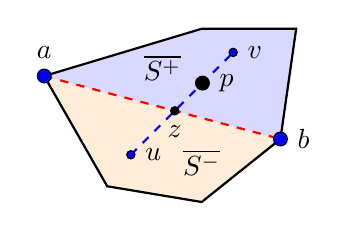
\begin{tikzpicture}
        \coordinate (a) at (0, 0.4);
        \coordinate (b) at (3, -0.4);
        \coordinate (v1) at (3.2, 1);
        \coordinate (v2) at (2, 1);
        \coordinate (u1) at (0.8, -1);
        \coordinate (u2) at (2, -1.2);
        \coordinate (u) at (1.1, -0.6);
        \coordinate (v) at (2.4, 0.7);
        \coordinate (p) at (2.01,0.31);
        \coordinate (z) at (1.65789, -0.0421053);

        \fill[blue, opacity=0.15] (b) -- (v1) -- (v2) -- (a) -- cycle;
        \fill[orange, opacity=0.15] (a) -- (u1) -- (u2) -- (b) -- cycle;

        \draw[thick] (a) -- (u1) -- (u2) -- (b) -- (v1) -- (v2) -- (a);
        \draw[dashed, thick, red] (a) -- (b);
        \draw[dashed, thick, blue] (u) -- (v);

        \node[draw, circle, black, fill=blue, inner sep=0pt, minimum size=5pt, label=above:$a$] (pA) at (a) {};
        \node[draw, circle, black, fill=blue, inner sep=0pt, minimum size=5pt, label=right:$b$] (pB) at (b) {};
        \node[draw, circle, black, fill=blue, inner sep=0pt, minimum size=3pt, label=right:$u$] (pU) at (u) {};
        \node[draw, circle, black, fill=blue, inner sep=0pt, minimum size=3pt, label=right:$v$] (pV) at (v) {};

        \node[draw, circle, black, fill=black, inner sep=0pt, minimum size=5pt, label=right:$p$] (pP) at (p) {};
        \node[draw, circle, black, fill=black, inner sep=0pt, minimum size=3pt, label=below:$z$] (pZ) at (z) {};

        \node[] at (1.5, 0.5) {$\overline{S^+}$};
        \node[] at (2, -0.7) {$\overline{S^-}$};

        \end{tikzpicture}
        \caption{}\label{fig:triangulation2-a}
    \end{subfigure}
    \begin{subfigure}{0.45\textwidth}
        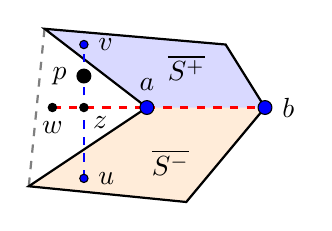
\begin{tikzpicture}
            \coordinate (a) at (1.5, 0);
            \coordinate (b) at (3, 0);
            \coordinate (v1) at (2.5, 0.8);
            \coordinate (v2) at (0.2, 1);
            \coordinate (u1) at (0, -1);
            \coordinate (u2) at (2, -1.2);
            \coordinate (u) at (0.7, -0.9);
            \coordinate (v) at (0.7, 0.8);
            \coordinate (p) at (0.7, 0.4);
            \coordinate (z) at (0.7, 0);
            \coordinate (w) at (0.3, 0);

            \fill[blue, opacity=0.15] (b) -- (v1) -- (v2) -- (a) -- cycle;
            \fill[orange, opacity=0.15] (a) -- (u1) -- (u2) -- (b) -- cycle;

            \draw[thick] (a) -- (u1) -- (u2) -- (b) -- (v1) -- (v2) -- (a);
            \draw[dashed, thick, red] (a) -- (b);
            \draw[dashed, thick, blue] (u) -- (v);
            \draw[dashed, thick, red] (w) -- (a);
            \draw[dashed, thick, opacity=0.5] (v2) -- (u1);

            \node[draw, circle, black, fill=blue, inner sep=0pt, minimum size=5pt, label=above:$a$] (pA) at (a) {};
            \node[draw, circle, black, fill=blue, inner sep=0pt, minimum size=5pt, label=right:$b$] (pB) at (b) {};
            \node[draw, circle, black, fill=blue, inner sep=0pt, minimum size=3pt, label=right:$u$] (pU) at (u) {};
            \node[draw, circle, black, fill=blue, inner sep=0pt, minimum size=3pt, label=right:$v$] (pV) at (v) {};

            \node[draw, circle, black, fill=black, inner sep=0pt, minimum size=5pt, label=left:$p$] (pP) at (p) {};
            \node[draw, circle, black, fill=black, inner sep=0pt, minimum size=3pt, label={[shift={(-0.05,0.05)}]-45:$z$}] (pZ) at (z) {};
            \node[draw, circle, black, fill=black, inner sep=0pt, minimum size=3pt, label=below:$w$] (pW) at (w) {};

            \node[] at (2, 0.5) {$\overline{S^+}$};
            \node[] at (1.8, -0.7) {$\overline{S^-}$};

        \end{tikzpicture}
        \caption{}\label{fig:triangulation2-b}
    \end{subfigure}
    \caption{Illustration of the proof for \lstinline|split_convexHull|. (a) Given point $p$, we obtain points $u$ and $v$ inside the two halves and $z$ as the point of intersection with the line $\overline{ab}$. (b) In this (contradictory) situation, the point $z$ has ended up outside the segment $\overline{ab}$, because $S$ is not actually convex. In this case we construct $w$ such that $z$ is on the $\overline{wa}$ segment, and observe that $w,z,a,b$ are collinear.}\label{fig:triangulation2}
\end{figure}
